\documentclass{scrbook}
\usepackage{graphicx} % Required for inserting images
\usepackage{tabularx} % Required for fixed width tables
\usepackage{scrlayer-scrpage} % Required for the subtitles
\usepackage{url} % Required for the URLs
\usepackage{hyperref} % Required for the URLs
\usepackage{listings} % Required for the code snippets
\usepackage{mathtools} % Required for the system of equations
\usepackage{amsmath,amssymb} % Required for some math symbols
\usepackage{enumitem} % Required for lettered lists

% Put the caption of the snippets at the bottom
\lstset{
    captionpos=b
}


\title{CoAP: Constrained Application Protocol}
\subtitle{Ambient intelligence course (A.Y. 2025/2026)\\Topic taught by Prof. Floriano Scioscia}
\author{Gabriele Colapinto}
\date{\today}

\begin{document}

\maketitle
\thispagestyle{empty}

{\Large\textbf{License}} \\
{Notes from Ambient intelligence (A.Y. 2025/2026) by Gabriele Colapinto. 
Course taught by professors Michele Ruta, Floriano Scioscia, Arnaldo Tomasino, Davide Loconte — 
Licensed under CC BY-NC 4.0.\\
\url{https://creativecommons.org/licenses/by-nc/4.0/}}

\vspace*{\fill}
\rule{\textwidth}{0.2pt}
\small{© 2025 Gabriele Colapinto \\
Released under the \href{https://creativecommons.org/licenses/by-nc/4.0/}{Creative Commons Attribution–NonCommercial 4.0 International License}}

\clearpage

\tableofcontents

\chapter{The Constrained Application Protocol (CoAP)}

This chapter explores the Constrained Application Protocol (CoAP), which represents a pragmatic engineering response to the inherent tension between the established web architecture and the severe resource constraints of IoT endpoints. As the digital and physical worlds become increasingly intertwined, a lightweight, efficient communication standard is paramount for the billions of small, embedded devices that will populate our environments. We will cover the rationale for CoAP's creation by examining the limitations of traditional web protocols in this new context. Furthermore, this chapter will detail CoAP's core design principles, deconstruct its highly efficient message structure, and analyze its distinct operational models, which ensure reliable communication over constrained and often unreliable networks.

\section{Context: From the Internet of Things to the Web of Things}

\begin{figure}
    \centering
    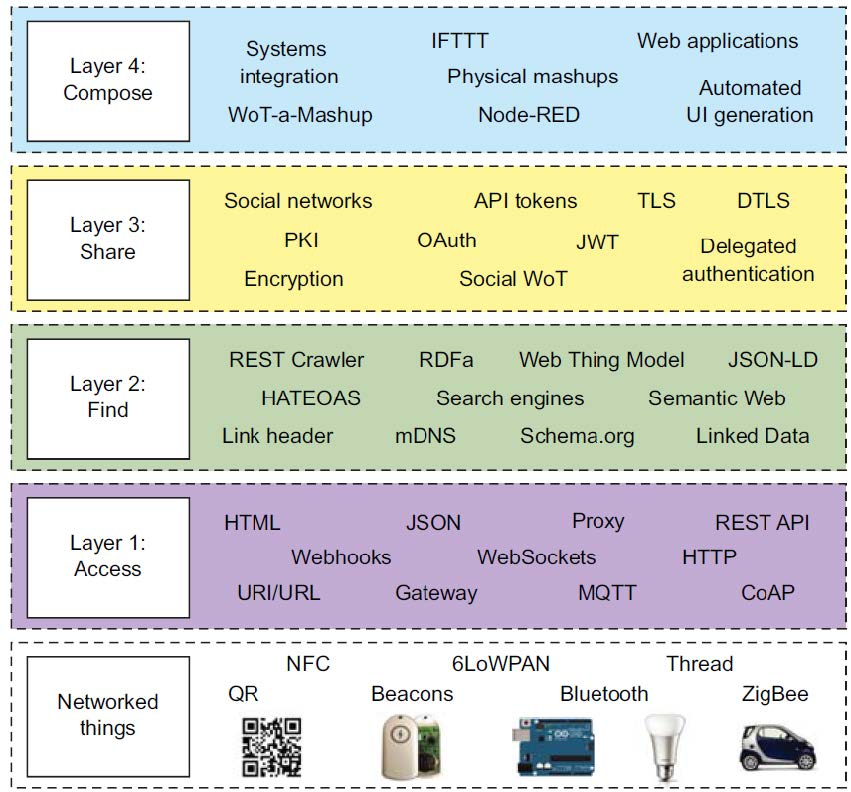
\includegraphics[width=0.5\linewidth]{Images/WoT_technologies.jpg}
    \caption{WoT technologies}
\end{figure}

The development of the Constrained Application Protocol (CoAP) is rooted in the strategic necessity of bridging the gap between the physical world of interconnected devices and the established digital ecosystem of the World Wide Web. This mission is the central focus of the \textbf{Web of Things (WoT)}, an initiative that seeks to create a seamless and interoperable environment where physical objects and web-based services can communicate and collaborate effectively.


The foundational vision is the \textbf{Internet of Things (IoT)}, which describes the embedding of internet connectivity directly into everyday objects, from simple sensors to complex industrial machinery. The IoT paradigm aims to make the internet accessible not just anytime and anywhere for anyone, but also for \textit{anything}.

Building upon this foundation, the \textbf{Web of Things (WoT)} seeks to be for the IoT what the World Wide Web is for the Internet. Its goal is to realize the IoT paradigm by applying standard, proven web technologies. By leveraging familiar tools like Uniform Resource Identifiers (URIs) for naming and the client-server model for interaction, the WoT aims to inherit the basic interoperability standards that made the web a global success.

However, this approach presents a fundamental challenge. While reusing established web protocols like the Hypertext Transfer Protocol (HTTP) is highly desirable for interoperability and ease of development, these protocols were designed for a very different environment. They are often ill-suited for the unique constraints of the low-power, memory-limited, and often intermittently connected devices that are typical in IoT deployments.

\section{Limitations of HTTP for Constrained Devices}

Directly applying HTTP to resource-constrained devices introduces several significant problems:

\begin{itemize}
    \item \textbf{Implementation Complexity:} The HTTP protocol specification is extensive, leading to complex implementations that demand significant Read-Only Memory (ROM) for code storage and Random-Access Memory (RAM) for operation. Many embedded devices simply do not have these resources.
    \item \textbf{Message Verbosity:} HTTP messages are text-based and verbose, which requires higher bandwidth to transmit. This is a critical issue in constrained networks, such as low-power wireless mesh networks, where bandwidth is a scarce and energy-intensive resource.
    \item \textbf{Interaction Model:} HTTP was primarily designed for human-driven interaction with web resources (e.g., a user browsing a website). While it can be adapted, its core design is not optimized for the autonomous, machine-to-machine (M2M) communication scenarios that dominate the IoT.
    \item \textbf{Feature Mismatch:} HTTP carries overhead for many features that are unneeded in M2M scenarios (e.g., cookies, complex headers) while lacking built-in, IoT-centric functionalities like resource discovery or an efficient event subscription model, which CoAP had to add.
\end{itemize}

To address these limitations, a purpose-built solution was needed—a protocol that could preserve the successful architectural principles of the web while being meticulously optimized for constrained environments. This solution is the Constrained Application Protocol.

\begin{figure}
    \centering
    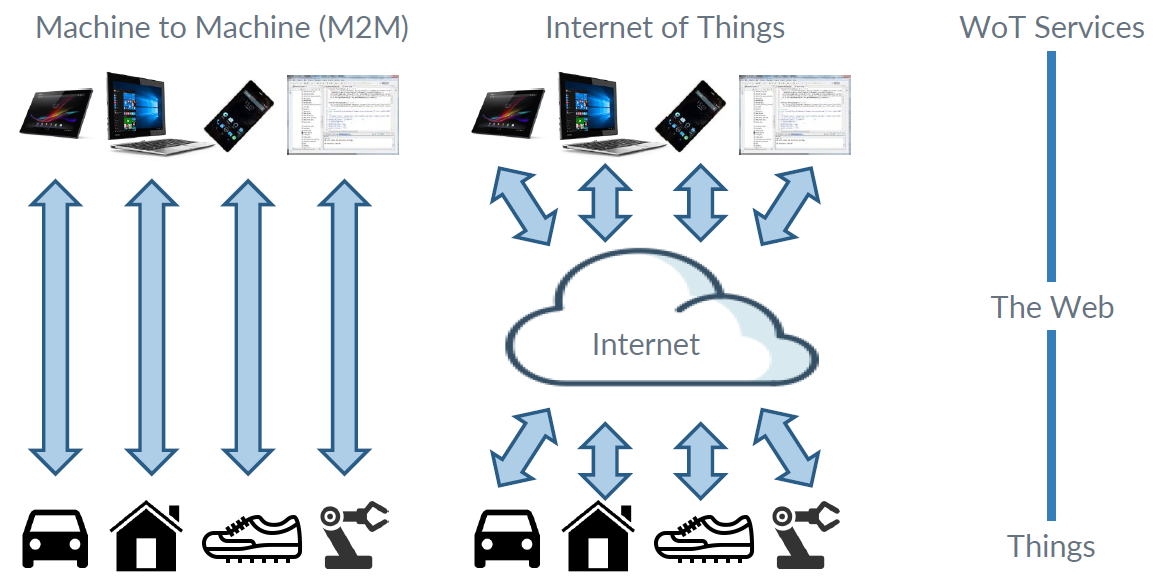
\includegraphics[width=0.5\linewidth]{Images/From_M2M_to_WoT.png}
    \caption{From M2M to WoT}
\end{figure}

\chapter{CoAP: A RESTful Protocol for a Constrained Web}

The Constrained Application Protocol (CoAP), defined in RFC 7252, is the specialized solution designed to overcome the challenges of applying traditional web protocols to the IoT. It acts as a practical and efficient bridge, connecting the world of standard HTTP-based web services with the low-power, resource-constrained devices that form the Web of Things. CoAP is not a replacement for HTTP but rather a compatible counterpart, enabling seamless communication across these two distinct technological domains.


At its core, CoAP is a \textbf{RESTful, HTTP-like protocol for resource-constrained pervasive objects}. By adhering to the principles of REST, CoAP's designers ensured that the protocol would inherit the scalability and architectural simplicity that made the World Wide Web successful, rather than attempting to invent a completely novel and unproven paradigm.

CoAP's architecture is founded on several key principles:

\begin{itemize}
    \item \textbf{Client-Server Model:} Like HTTP, CoAP operates on a stateless request-response model. Clients make requests to servers to manipulate resources (e.g., read a sensor value, actuate a switch).
    \item \textbf{HTTP Semantics:} It inherits the concept of resources and the basic methods used to interact with them: \texttt{GET}, \texttt{POST}, \texttt{PUT}, and \texttt{DELETE}. This semantic alignment simplifies the logic for developers familiar with web development.
    \item \textbf{Gateway Compatibility:} CoAP was explicitly designed to be mapped to and from HTTP. This is a critical design feature, as it allows for the creation of "cross-proxies" or gateways that translate between the two protocols. This enables the billions of future CoAP devices to be first-class citizens of the existing web, accessible via standard HTTP requests from any browser or web service without requiring the client to understand CoAP. This seamless integration is the core enabler of the WoT vision.
    \item \textbf{Lightweight Transport:} Instead of the connection-oriented and relatively heavy Transmission Control Protocol (TCP) used by HTTP, CoAP is built upon the User Datagram Protocol (UDP). This represents a crucial engineering trade-off: CoAP forgoes the significant overhead of a TCP handshake and connection management in favor of a tailored, "good enough" reliability mechanism at the application layer, which is a far more efficient model for short-lived, sporadic IoT transactions.
    \item \textbf{Application-Layer Reliability:} Since UDP is an unreliable transport protocol, CoAP implements its own basic reliability mechanisms at the application level. This ensures that important messages are acknowledged without the complexity and resource cost of a full TCP stack.
\end{itemize}

These principles were guided by a specific set of design requirements that directly address the realities of building a functional and robust Web of Things.

\chapter{CoAP Design Requirements}

\begin{figure}
    \centering
    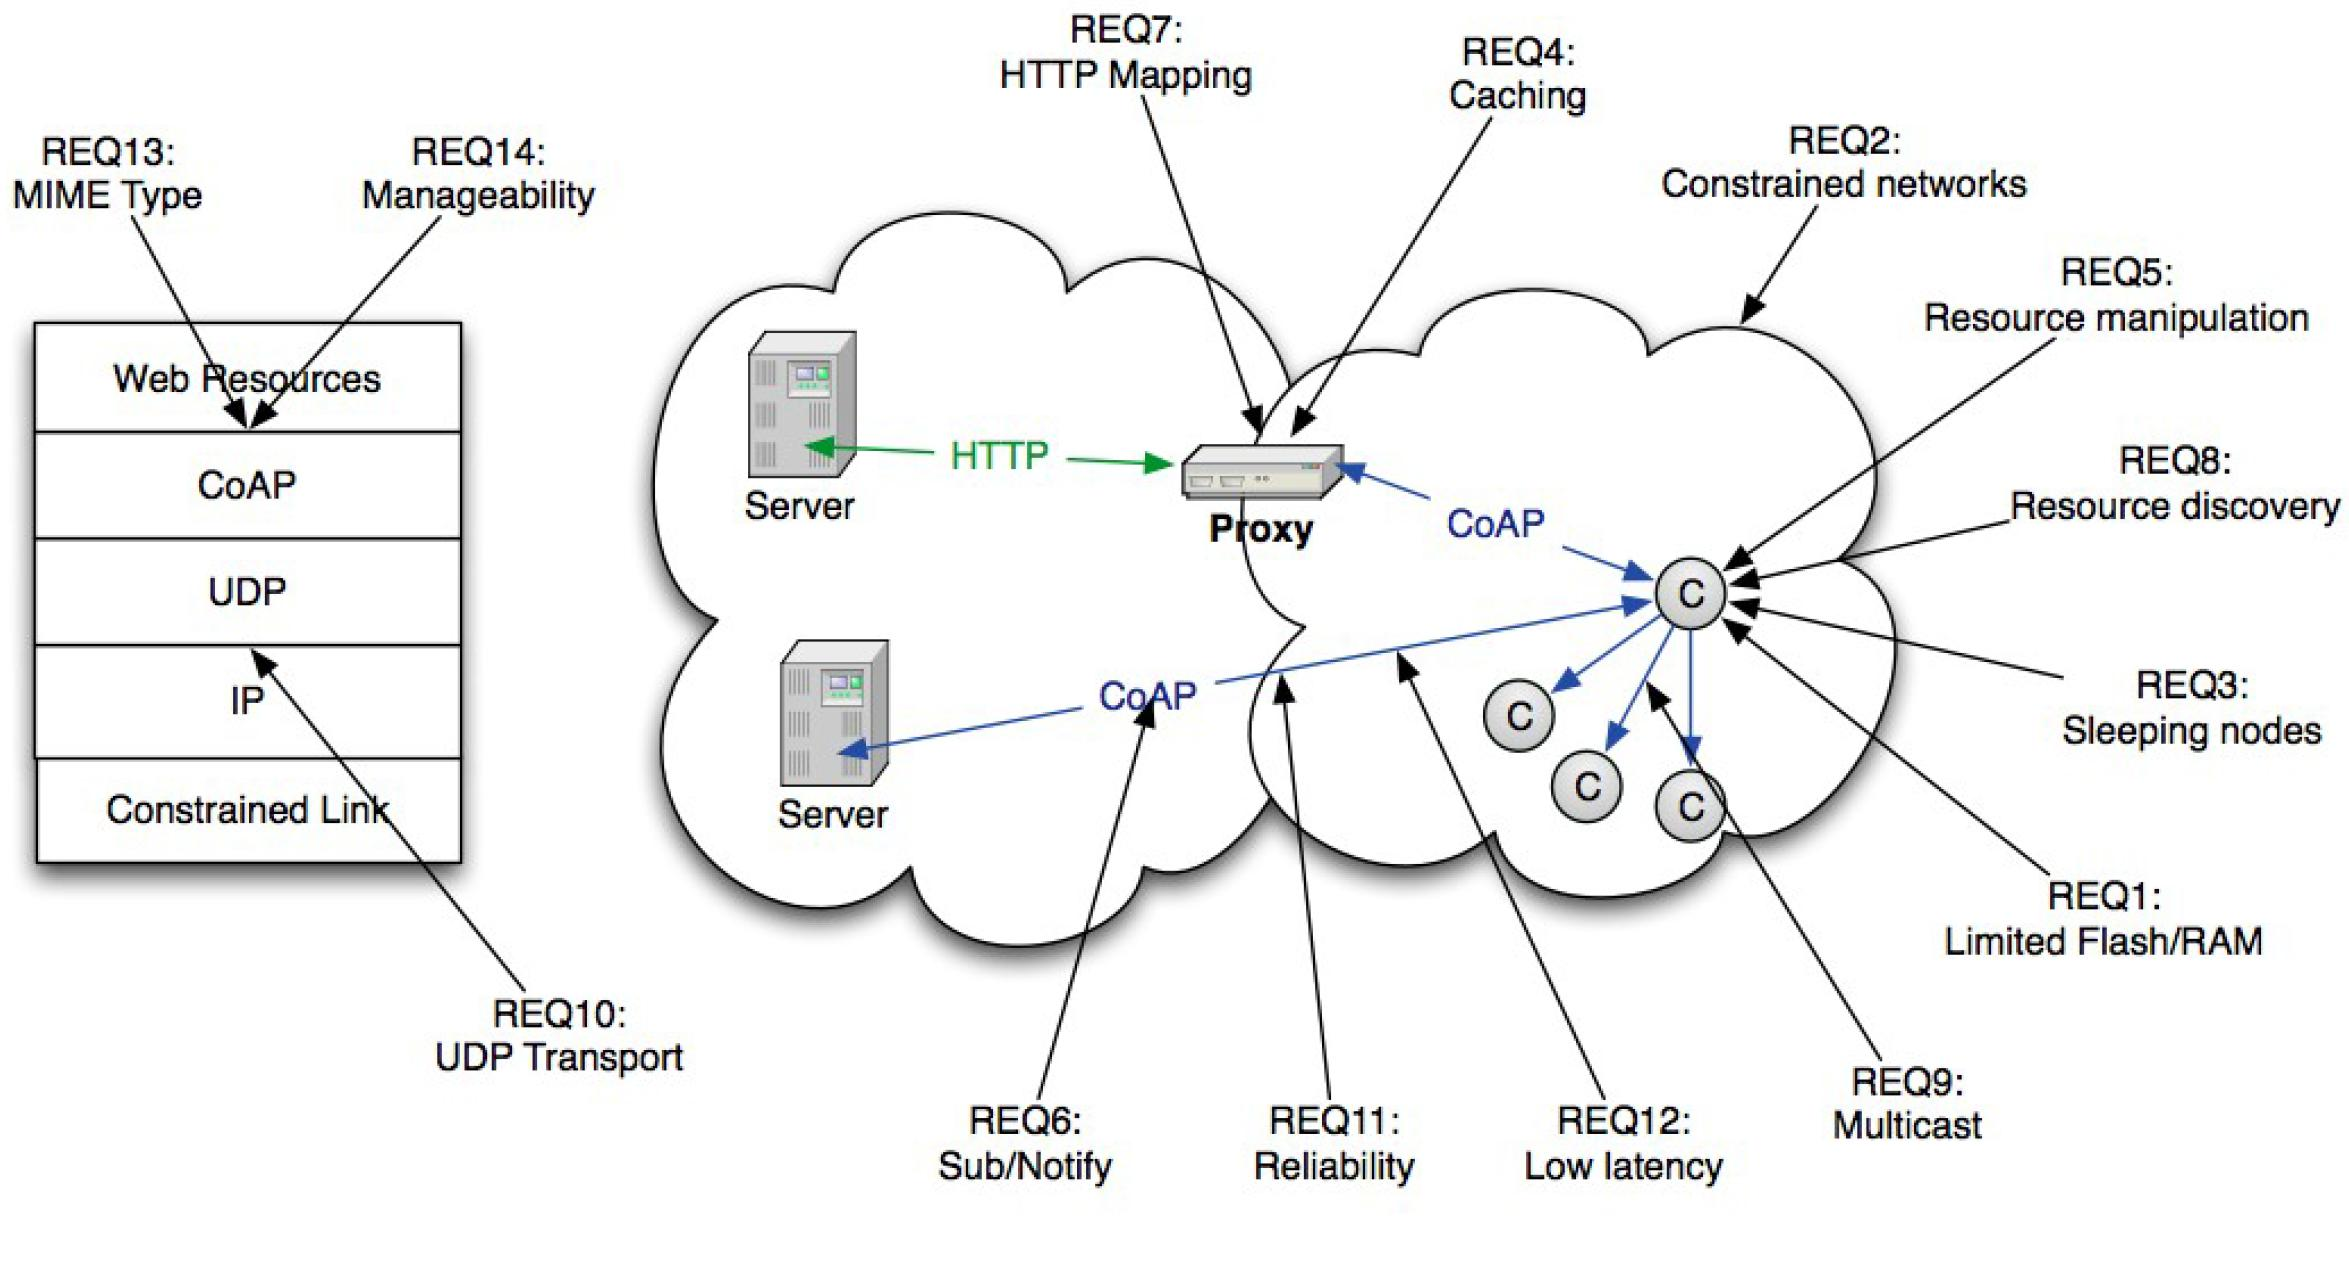
\includegraphics[width=\linewidth]{Images/CoAP_design_requirements.jpg}
    \caption{CoAP design requirements}
\end{figure}

The design of CoAP was not arbitrary but was driven by a specific set of requirements tailored to the unique challenges of constrained networks and devices. These foundational requirements shaped the protocol's features, ensuring its suitability for real-world IoT applications where efficiency and robustness are paramount.

\begin{enumerate}
    \item \textbf{Low Message Overhead:} To conserve memory, processing power, and energy, messages must have a minimal header size and be simple to parse. This requirement directly led to CoAP's compact binary header and efficient option encoding.
    \item \textbf{URI and HTTP Mapping:} The protocol must integrate seamlessly with the existing web. This requires a straightforward way to map CoAP Uniform Resource Identifiers (URIs) and methods to their HTTP equivalents, enabling the cross-proxies that bridge the two ecosystems.
    \item \textbf{Support for Constrained Networks:} CoAP is designed to function effectively over low-bandwidth, high-latency, and lossy networks. It must also accommodate devices that sleep for long periods to conserve energy or have intermittent connectivity, which is a common operational state in many IoT deployments.
    \item \textbf{Resource Discovery:} In a typical web environment, users rely on search engines to discover resources. In an M2M context, devices need an automated, built-in mechanism to discover the resources available on other devices on the network. CoAP provides this capability.
    \item \textbf{Multicast Support:} A key requirement for many IoT scenarios is the ability to communicate with groups of devices simultaneously. CoAP supports multicast, allowing a single request to be sent to a set of devices, for example, to turn on all the lights in a room with one command.
    \item \textbf{Observation Support:} Constantly polling a sensor for updates is highly inefficient and drains battery life, especially over lossy networks. To address this, CoAP includes a built-in subscription model, allowing a client to "observe" a resource. The server will then proactively notify the client whenever the state of that resource changes, eliminating wasteful polling.
\end{enumerate}

These requirements directly influenced the design of CoAP's message architecture, which is engineered for maximum efficiency.

\chapter{The CoAP Message Architecture}

A cornerstone of CoAP's design is its compact, binary message format. This is a direct answer to the 'Low Message Overhead' requirement discussed previously and stands in stark contrast to HTTP's verbose, text-based format. Every byte in a CoAP message is carefully allocated to minimize overhead, reduce parsing complexity, and conserve network bandwidth. The following subsections deconstruct the CoAP message to show how it achieves this remarkable level of optimization.


\section{General Message Structure}

\begin{figure}
    \centering
    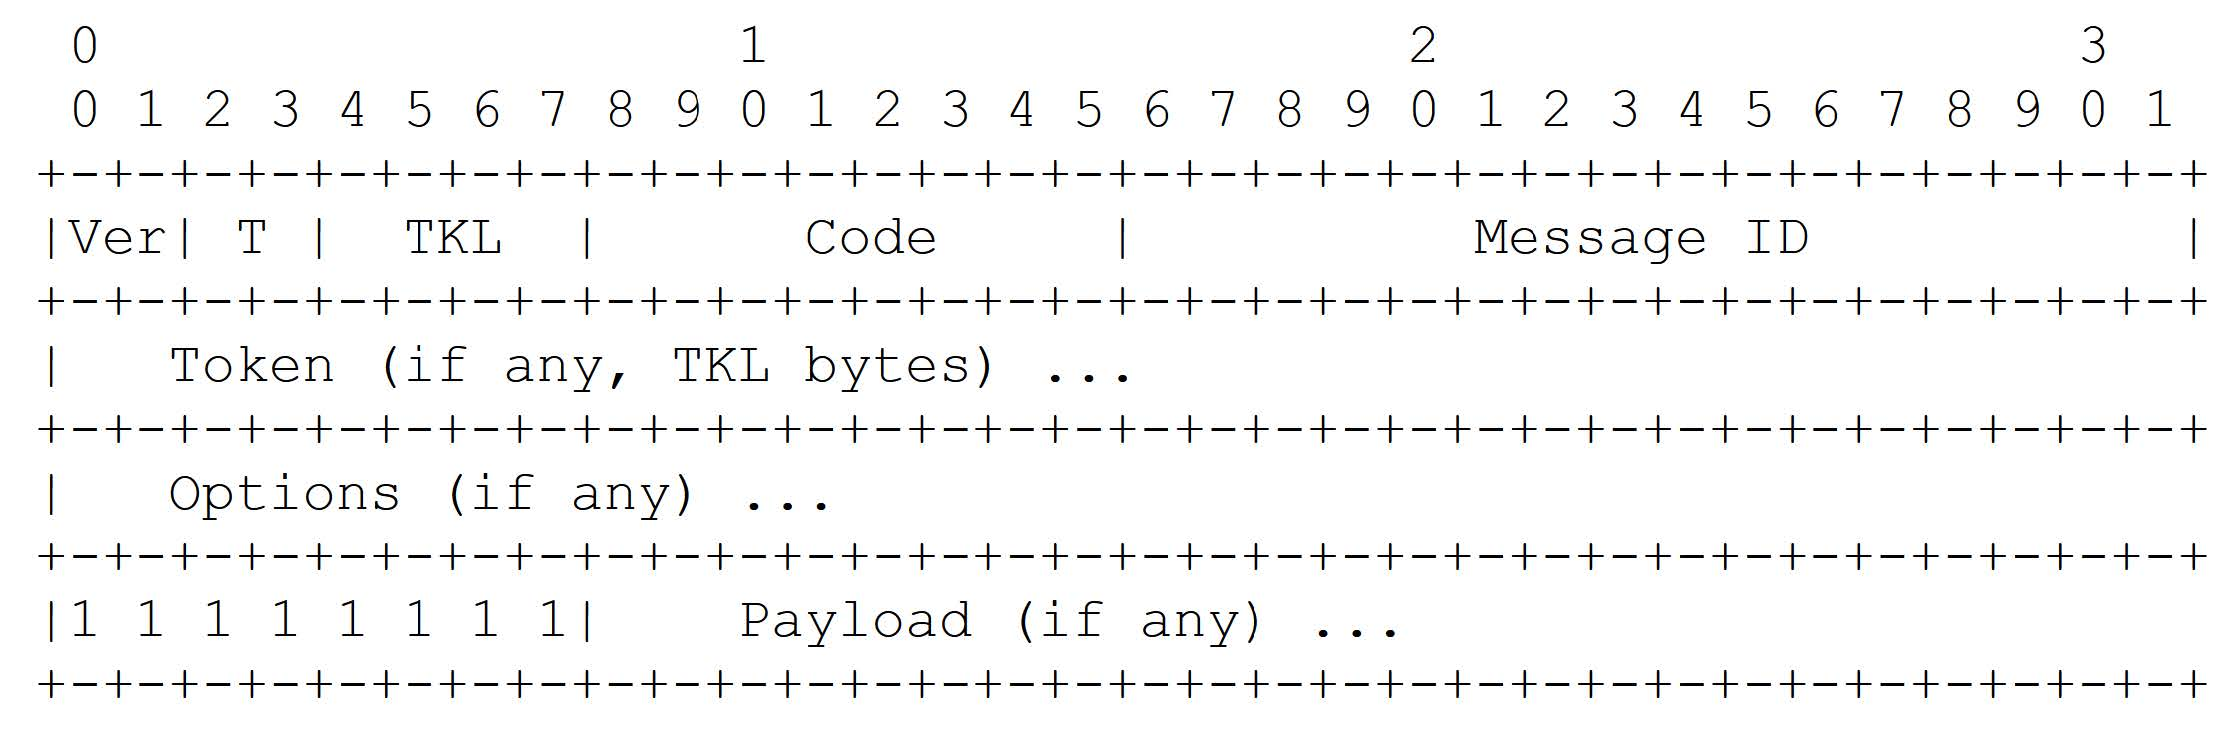
\includegraphics[width=\linewidth]{Images/CoAP_message_structure.jpg}
    \caption{CoAP message structure}
\end{figure}

Every CoAP message consists of up to four primary components arranged in a specific sequence. This structure provides a fixed, easy-to-parse preamble followed by optional fields for more complex interactions.

\begin{itemize}
    \item \textbf{Fixed Header:} A mandatory 4-byte header that contains essential control information, such as the CoAP version, message type, and message ID.
    \item \textbf{Token:} An optional sequence of 0 to 8 bytes used to correlate a request with its corresponding response.
    \item \textbf{Options:} An optional sequence of one or more options that function like lightweight HTTP headers, carrying information such as the target URI path or content format.
    \item \textbf{Payload Separator \& Payload:} If the message carries a data payload (e.g., a sensor reading or a command), it is preceded by a fixed one-byte separator (\texttt{11111111}). The payload itself is optional.
\end{itemize}

\section{Deconstructing the CoAP Header}

\begin{figure}
    \centering
    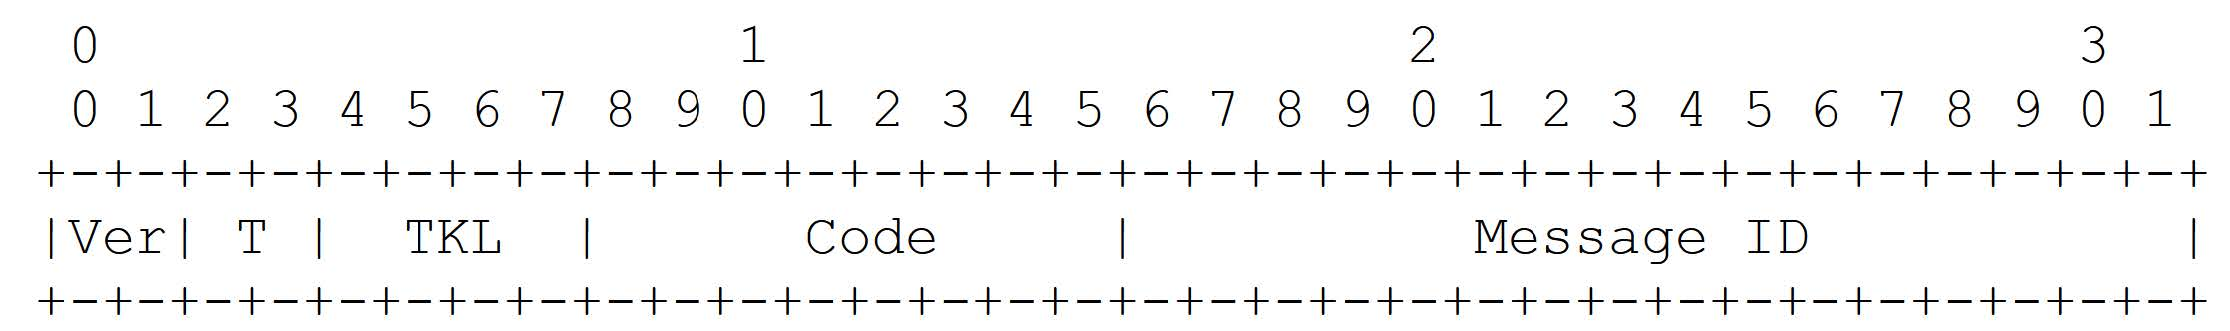
\includegraphics[width=\linewidth]{Images/CoAP_header.jpg}
    \caption{CoAP header}
\end{figure}

The fixed 4-byte header is the core of every CoAP message, providing the fundamental information needed to process it. Its fields (exposed in table 4.1) are tightly packed to convey maximum information in a minimal space.

\begin{table}[h]
    \centering
    \begin{tabular}{|l|p{2cm}|p{8cm}|}
    \hline
    \textbf{Field} & \textbf{Size (bits)} & \textbf{Description} \\
    \hline
    \textbf{Ver} & 2 & The CoAP version number. The current version is \texttt{1}. \\
    \hline
    \textbf{T} & 2 & The message \textbf{T}ype: \texttt{Confirmable}, \texttt{Non-confirmable}, \texttt{Acknowledgment}, or \texttt{Reset}. \\
    \hline
    \textbf{TKL} & 4 & The \textbf{T}o\textbf{k}en \textbf{L}ength, specifying the length of the following Token field in bytes (from 0 to 8). \\
    \hline
    \textbf{Code} & 8 & Indicates the request method (see figure 4.3) or the response code (see figure 4.4), divided into a 3-bit class (e.g., 0 for request, 2 for success, 4 for client error and 5 for server error) and a 5-bit detail containing one of the possible values in CoAP Code Registries. \\
    \hline
    \textbf{Message ID} & 16 & A unique ID used for message deduplication and to match \texttt{Acknowledgment} messages with their corresponding \texttt{Confirmable} messages. \\
    \hline
    \end{tabular}
    \caption{CoAP Header Structure}
\end{table}

\begin{figure}
    \centering
    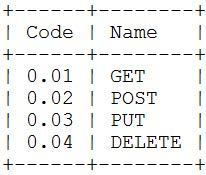
\includegraphics[width=0.5\linewidth]{Images/Methods.jpg}
    \caption{CoAP request method codes - There is also a special code 0.00 for empty messages}
\end{figure}

\begin{figure}
    \centering
    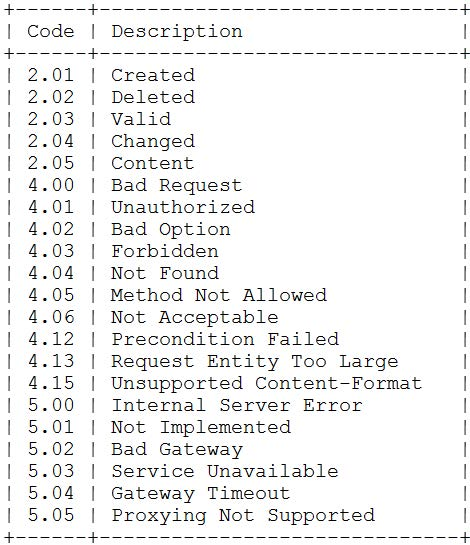
\includegraphics[width=0.5\linewidth]{Images/Responses.jpg}
    \caption{CoAP response codes}
\end{figure}

\chapter{Understanding CoAP Options and Delta Encoding}

The Constrained Application Protocol (CoAP) provides a compact and efficient alternative to HTTP, specifically designed for constrained devices and low-power, lossy networks. One of the key elements enabling this efficiency is the use of \emph{options}, which represent metadata in a structured binary format rather than as verbose textual headers.

Unlike HTTP, CoAP does not transmit a complete textual URI or header fields. Instead, all request metadata is encoded as a sequence of typed options, each identified by a numeric \emph{Option Number}. This design allows CoAP to minimize message size while preserving expressiveness and extensibility.

\section{Option Numbers and Delta Encoding}

Each CoAP option is associated with a well-known numeric identifier called the \emph{Option Number}. Rather than encoding the full option number for every option, CoAP uses a \textbf{delta encoding} mechanism. Options are transmitted in \textbf{strictly increasing order} of their option numbers, and each option carries only the numerical difference (delta) with respect to the previous option.

Formally, if $O_i$ is the option number of the $i$-th option, the encoded delta is:

\[
\Delta_i = O_i - O_{i-1}
\]

with $O_0 = 0$.

This mechanism significantly reduces the number of bits required to represent option identifiers, as commonly used options have small and closely spaced numeric values.

\section{Structure of a CoAP Option}

\begin{figure}
    \centering
    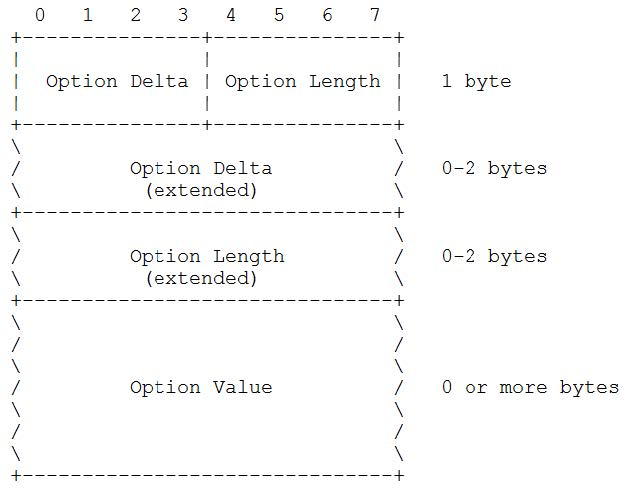
\includegraphics[width=0.5\linewidth]{Images/Option_format.jpg}
    \caption{CoAP option structure}
\end{figure}

Each option in a CoAP message consists of three logical fields:

\begin{itemize}
    \item \textbf{Option Delta}: the difference between the current option number and the previous one;
    \item \textbf{Option Length}: the length, in bytes, of the option value;
    \item \textbf{Option Value}: the data associated with the option.
\end{itemize}

The Option Delta and Option Length fields are encoded together in a single byte, using 4 bits each. Values from 0 to 12 are encoded directly, while larger values use an extended encoding scheme. Certain bit patterns are reserved to signal malformed options, allowing invalid messages to be detected early.

\section{Stateless Parsing of Options}

Although delta encoding relies on the previous option number, CoAP remains a strictly \emph{stateless} protocol. The receiver does not store information from previous messages. Instead, it reconstructs the option numbers incrementally while parsing a single message.

Upon receiving a message, the receiver initializes a local variable storing the current option number, for instance:

\[
\texttt{current\_option\_number} = 0
\]

For each option, the receiver adds the received delta to this local variable to obtain the actual option number. This process occurs entirely within the scope of the current message and requires no persistent state across requests.

This design allows CoAP to combine compact encoding with stateless operation, which is essential for scalability and robustness in constrained environments.

\section{URI Representation Through Options}

CoAP does not transmit a URI as a single string. Instead, it decomposes the URI into its constituent components, each encoded as a separate option. The primary URI-related options are:

\begin{itemize}
    \item \texttt{Uri-Host} (Option Number 3)
    \item \texttt{Uri-Port} (Option Number 7)
    \item \texttt{Uri-Path} (Option Number 11, repeatable)
    \item \texttt{Uri-Query} (Option Number 15, repeatable)
\end{itemize}

For example, the path \texttt{/sensors/temperature} is encoded as two separate \texttt{Uri-Path} options, one for each path segment. Repeated options are permitted because they share the same option number; in such cases, the encoded delta is zero. 

\section{Example: Encoding a GET Request Using Options}

Consider the HTTP request:

\begin{verbatim}
    GET http://example.com:400/sensors/temperature?unit=celsius&precision=high
\end{verbatim}

When translated into CoAP options, the logical option sequence is:

\begin{itemize}
    \item \texttt{Uri-Host = example.com}
    \item \texttt{Uri-Port = 400}
    \item \texttt{Uri-Path = sensors}
    \item \texttt{Uri-Path = temperature}
    \item \texttt{Uri-Query = unit=celsius}
    \item \texttt{Uri-Query = precision=high}
\end{itemize}

The corresponding option numbers and deltas are shown in Table~\ref{tab:coap-delta-example}.

\begin{table}[h]
    \centering
    \begin{tabular}{|c|c|c|}
        \hline
        \textbf{Option} & \textbf{Option Number} & \textbf{Delta} \\
        \hline
        Uri-Host & $3$ & $3 - 0 = (3)_{10} = (11)_2 \rightarrow 2$ bits \\
        Uri-Port & $7$ & $7 - 3 = (4)_{10} = (100)_2 \rightarrow 3$ bits \\
        Uri-Path & $11$ & $11 - 7 = (4)_{10} = (100)_2 \rightarrow 3$ bits \\
        Uri-Path & $11$ & $11 - 11 = (0)_{10} = (0)_2 \rightarrow 1$ bit \\
        Uri-Query & $15$ & $15 - 11 = (4)_{10} = (100)_2 \rightarrow 3$ bits \\
        Uri-Query & $15$ & $15 - 15 = (0)_{10} = (0)_2 \rightarrow 1$ bit \\
        \hline
    \end{tabular}
    \caption{Delta encoding of CoAP options for a GET request}
    \label{tab:coap-delta-example}
\end{table}

Only the delta values are transmitted in the message. The receiver reconstructs the full option numbers incrementally during parsing. \\

This example is also useful to expose why some options are repeatable.
The Uri-Host and Uri-Port are not repeatable because we make a request to a single machine and a single port. Once the request reached the port of the machine, the client has to specify what it wants and how it wants it. As for the first requirement, the GET request has to specify the path steps to reach the resource one at a time. So, the Uri-Path has to be a repeatable option to navigate the file system of the server. As for the second requirement, the Uri-Query is a repeatable option because it must be possible to specify more than one feature of the requested resource. In this example we specify the temperature unit and precision but in other cases we could specify other features of the data. For example, let's say that we have a building whose windows have sensor to check if they are opened or closed, they have a unique identifier and are associated to their floor. Let's say that all those sensors are linked to a CoAP device and we want the list of IDs of the opened windows of the second floor. In this case our request would be:

\begin{verbatim}
    GET http://company.building.com:123/sensors/windows?status=open&floor=2
\end{verbatim}

\section{Why Options Are Always Present}

Although all CoAP requests follow the same general structure, the \texttt{Options} field is essential because it conveys the semantic meaning of the request. The server does not infer resource identifiers implicitly; instead, it relies exclusively on the received options to determine the target resource and request parameters.

This explicit representation allows:
\begin{itemize}
    \item stateless processing;
    \item efficient routing and proxying;
    \item flexible extension of the protocol without breaking compatibility.
\end{itemize}

\section{Error Detection Through CoAP Options}

The structured representation of metadata through CoAP options not only enables compact encoding, but also plays a crucial role in the early detection of malformed or invalid requests. Errors in a CoAP request can be broadly classified into syntactic errors and semantic errors. Each category can be identified at a different stage of message processing.

\subsection{Syntactic Errors}

Syntactic errors arise when the binary structure of the message violates the CoAP message format. These errors can be detected during the low-level parsing of the message, before any application logic is involved.

Typical syntactic errors include:

\begin{itemize}
    \item invalid option delta or option length encodings (e.g., reserved 4-bit values);
    \item truncated option values that do not match the declared option length;
    \item options appearing out of order, resulting in a reconstructed option number smaller than the previous one;
    \item malformed message structure, such as missing mandatory fields or incorrect payload markers.
\end{itemize}

Because options are encoded sequentially and deltas must always be non-negative, many malformed messages can be detected immediately during option parsing, allowing the receiver to discard the request with minimal processing overhead.

\subsection{Semantic Errors in Options}

Semantic errors occur when the message is syntactically well-formed but contains option values or combinations that are invalid according to the CoAP specification.

Examples of semantic errors include:

\begin{itemize}
    \item the presence of an option that is not allowed for the given request method;
    \item an option appearing more times than permitted by the specification;
    \item mutually exclusive options being used together;
    \item option values that violate constraints defined by the option semantics (e.g., invalid port numbers or malformed query strings).
\end{itemize}

Since each option has a well-defined numeric identifier and semantics, the receiver can validate each reconstructed option number against the set of known options and their rules. Unknown options are handled according to their \emph{critical} or \emph{elective} nature, as specified by the protocol.

\section{CoAP Option Flags and Semantics}

\begin{figure}
    \centering
    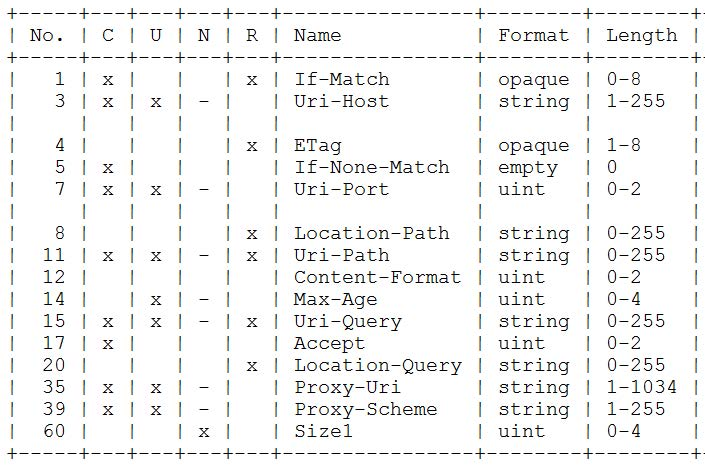
\includegraphics[width=\linewidth]{Images/Options.jpg}
    \caption{CoAP options flags}
    \label{fig:coap_option_flags}
\end{figure}

Each CoAP option is identified not only by its numeric Option Number, but also by a set of semantic properties encoded implicitly in specific bits of that number. These properties, commonly referred to as \emph{option flags}, determine how an option must be handled by intermediaries and endpoints.

Unlike explicit header fields, CoAP does not transmit option flags separately. Instead, the flags are derived from the binary structure of the Option Number itself, ensuring compactness and efficient processing.

\subsection{Critical vs Elective Options}

The most significant property of a CoAP option is whether it is \textbf{critical} or \textbf{elective}. This distinction determines how a receiver must behave when it encounters an unknown option.

\begin{itemize}
    \item An option is \textbf{critical} if it is essential for correctly understanding the request or response semantics.
    \item An option is \textbf{elective} if it provides additional information that can be safely ignored without altering the core meaning of the message.
\end{itemize}

If a receiver encounters an unknown \textbf{critical} option, it must reject the message and respond with an error. Conversely, unknown \textbf{elective} options may be ignored.

\paragraph{How Criticality Is Determined}

Criticality is not an independent field. It is determined by the least significant bit of the Option Number:

\begin{itemize}
    \item odd Option Numbers $\Rightarrow$ \textbf{critical} options;
    \item even Option Numbers $\Rightarrow$ \textbf{elective} options.
\end{itemize}

Therefore, if the critical flag is \texttt{false}, the option is automatically elective. There is no third category.

\subsection{Unsafe and NoCacheKey Flags}

Additional properties of options are encoded in higher-order bits of the Option Number and control how proxies and caches handle the message.

\begin{itemize}
    \item The \textbf{Unsafe} flag indicates whether an option may affect the semantics of a request when forwarded by a proxy. Unsafe options require careful handling and may prevent certain optimizations.
    \item The \textbf{NoCacheKey} flag indicates whether an option should be excluded from cache key calculations.
\end{itemize}

An option marked as unsafe or excluded from cache keys influences how intermediaries cache and forward messages, but does not affect the endpoint’s ability to interpret the request.

\subsection{Repeatable Options}

The \textbf{Repeatable} property specifies whether an option may appear multiple times in the same message.

\begin{itemize}
    \item \textbf{Repeatable} options may occur more than once, with each occurrence contributing to the overall semantics.
    \item \textbf{Non-repeatable} options must appear at most once; multiple occurrences constitute a semantic error.
\end{itemize}

Typical examples of repeatable options include \texttt{Uri-Path} and \texttt{Uri-Query}, which naturally consist of multiple components.

\subsection{Choosing Option Properties}

The choice of these properties is determined at protocol design time, not by the sender or receiver. Each option defined by the CoAP specification or by an extension explicitly assigns its semantic role.

In particular:

\begin{itemize}
    \item options that affect resource identification are typically critical;
    \item options that provide auxiliary metadata are often elective;
    \item options that influence proxy behavior tend to be unsafe;
    \item options representing segmented structures are usually repeatable.
\end{itemize}

This design ensures forward compatibility while preserving protocol correctness.

\subsection{Uri-Path vs Location-Path}

Although \texttt{Uri-Path} and \texttt{Location-Path} have similar structures, they serve distinct purposes.

\begin{itemize}
    \item \texttt{Uri-Path} is used in requests to identify the target resource.
    \item \texttt{Location-Path} is used in responses to indicate the location of a newly created resource.
\end{itemize}

For example, after a successful \texttt{POST} request that creates a new resource, the server may include \texttt{Location-Path} options to inform the client where the resource can be accessed.

\subsection{Uri-Query vs Location-Query}

Similarly, \texttt{Uri-Query} and \texttt{Location-Query} are semantically distinct:

\begin{itemize}
    \item \texttt{Uri-Query} refines a request by supplying query parameters.
    \item \texttt{Location-Query} provides additional query components associated with a resource location in a response.
\end{itemize}

Location-related options are never used for request interpretation; they are purely informative and appear only in responses.

\section{Option Value Formats}

While all CoAP options share the same structural encoding—consisting of an option delta, an option length, and an option value—the interpretation of the option value depends on the \emph{option format}. The option format specifies how the sequence of bytes carried in the option value must be interpreted by the receiver.

It is important to note that the option format is \emph{not} explicitly encoded in the message. Instead, it is implicitly defined by the option number itself, as specified in the CoAP standard or in an extension specification. The receiver determines the format by recognizing the option number.

CoAP defines four conceptual formats for option values: \texttt{opaque}, \texttt{string}, \texttt{uint}, and \texttt{empty}.

\subsection{Opaque Format}

An option with format \texttt{opaque} carries an uninterpreted sequence of bytes. From the perspective of the CoAP protocol, the content of the option value has no internal structure or semantic meaning.

In particular:
\begin{itemize}
    \item no character encoding is assumed;
    \item no numeric interpretation is imposed;
    \item no byte order (endianness) is defined by the protocol.
\end{itemize}

The option value is treated purely as a binary blob. Any interpretation of the bytes is entirely delegated to the entity that defines or uses the option, such as an application-level protocol or an extension specification.

If an opaque option value represents structured data (for example, a numeric identifier or a hash), the interpretation rules—including byte ordering—must be defined externally. They must not depend on the underlying hardware architecture, in order to preserve interoperability between heterogeneous devices.

Typical examples of opaque options include \texttt{ETag} and \texttt{If-Match}, which are compared byte-by-byte without any semantic interpretation by the protocol.

\subsection{String Format}

Options with format \texttt{string} carry a textual value encoded as a UTF-8 string. The length of the string is determined by the option length field, and no null terminator is included.

The string format is commonly used for options that represent human-readable components, such as URI elements. Examples include:

\begin{itemize}
    \item \texttt{Uri-Host}
    \item \texttt{Uri-Path}
    \item \texttt{Uri-Query}
    \item \texttt{Location-Path}
\end{itemize}

The receiver interprets the option value as a UTF-8 encoded string and may perform semantic validation based on the option definition.

\subsection{Unsigned Integer Format (\texttt{uint})}

The \texttt{uint} format represents a non-negative integer encoded in network byte order (big-endian). The length of the encoding is variable and ranges from zero to four bytes.

A length of zero encodes the value zero. No padding bytes are allowed, ensuring a canonical representation of integer values.

The \texttt{uint} format is used whenever an option semantically represents a numeric quantity that must be interpreted consistently across different implementations. Examples include:

\begin{itemize}
    \item \texttt{Uri-Port}
    \item \texttt{Max-Age}
    \item \texttt{Content-Format}
\end{itemize}

By defining a fixed byte order and representation, the \texttt{uint} format avoids ambiguity and simplifies validation.

\subsection{Empty Format}

The \texttt{empty} format denotes an option that carries no value. Its option length is zero, and no option value bytes are present.

The semantic meaning of an empty option is conveyed solely by its presence in the message. Such options are typically used to modify the behavior of a request rather than to transmit data.

A notable example is \texttt{If-None-Match}, which signals a conditional request without requiring an explicit value.

\subsection{Rationale for Multiple Formats}

The introduction of distinct option formats serves several purposes:

\begin{itemize}
    \item it enables efficient and unambiguous parsing;
    \item it avoids unnecessary textual representations of numeric values;
    \item it supports extensibility through opaque values;
    \item it allows early detection of semantic errors.
\end{itemize}

In particular, the distinction between \texttt{opaque} and \texttt{uint} is crucial. While both formats are transmitted as raw bytes, only \texttt{uint} defines a canonical numeric interpretation. The \texttt{opaque} format intentionally avoids imposing any structure, leaving interpretation entirely outside the scope of the CoAP protocol.

\section{Summary}

In summary, CoAP encodes both the structure and semantics of options in a highly compact form. Option formats define how option value bytes are to be interpreted, even though they are always transmitted as raw octets, while option flags—implicitly derived from option numbers—govern extensibility, error handling, and proxy behavior. By combining a small set of well-defined value formats with semantic properties encoded directly into option numbers, CoAP achieves an effective balance between efficiency, simplicity, robustness, and extensibility, making it particularly well suited for interoperable IoT systems.

\chapter{CoAP Interaction Models and Reliability}

CoAP operates over the unreliable UDP transport layer, which means it cannot take packet delivery for granted. To provide robust communication, CoAP implements its own lightweight reliability mechanisms and offers two primary models for request-response interactions: the \textbf{piggybacked response} and the \textbf{separate response}. These models allow CoAP to balance efficiency with the potential for processing delays on the server side, ensuring it can adapt to different application needs. This chapter explores these models and the underlying mechanisms that make them possible.

\section{Message Types and Reliability Mechanism}

CoAP defines four message types that are fundamental to its operation and reliability:

\begin{itemize}
    \item \textbf{Confirmable (CON):} An important message that requires an Acknowledgment (ACK) from the recipient. If an ACK is not received, the sender will retransmit the message.
    \item \textbf{Non-confirmable (NON):} A "fire-and-forget" message that does not require an ACK. This is suitable for repetitive sensor readings or other data where the loss of a single message is acceptable.
    \item \textbf{Acknowledgment (ACK):} Confirms the receipt of a CON message. In the piggybacked model, this message also carries the full response payload.
    \item \textbf{Reset (RST):} A message sent in reply to a CON or NON message to indicate that the received message was not processable (e.g., the recipient was not prepared to handle it).
\end{itemize}

The core reliability mechanism is simple yet effective: when a sender transmits a \textbf{CON} message, it starts a timeout. If it does not receive a corresponding \textbf{ACK} before the timeout expires, it assumes the packet was lost and retransmits the \textit{exact same message} with the \textit{exact same Message ID}. This Message ID is critical, as it allows the receiver to detect and discard any duplicate messages it might receive due to retransmissions.

\section{The Piggybacked Response Model}

\begin{figure}
    \centering
    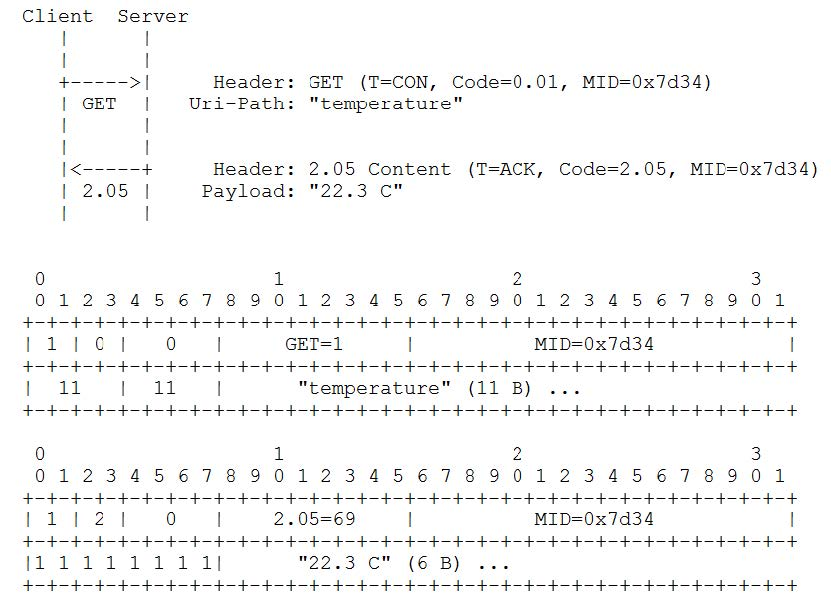
\includegraphics[width=\linewidth]{Images/Piggybacked response.jpg}
    \caption{Piggybacked response}
\end{figure}

The piggybacked response is the most common and efficient interaction model in CoAP. It is used when the server can generate a response immediately upon receiving a request.


The process is straightforward:

\begin{enumerate}
    \item A client sends a request as a \textbf{CON} message.
    \item The server receives the request and processes it quickly.
    \item The server sends its response back to the client. Instead of sending a separate response message, it places the response data directly inside the \textbf{ACK} message it must send to confirm the client's CON request.
\end{enumerate}

In this model, the server's response message has the type \textbf{ACK} and carries the \textit{same Message ID} as the client's original request. This elegantly combines the transport-layer acknowledgment with the application-layer response into a single, highly efficient message exchange.

\section{The Separate Response Model}

\begin{figure}
    \centering
    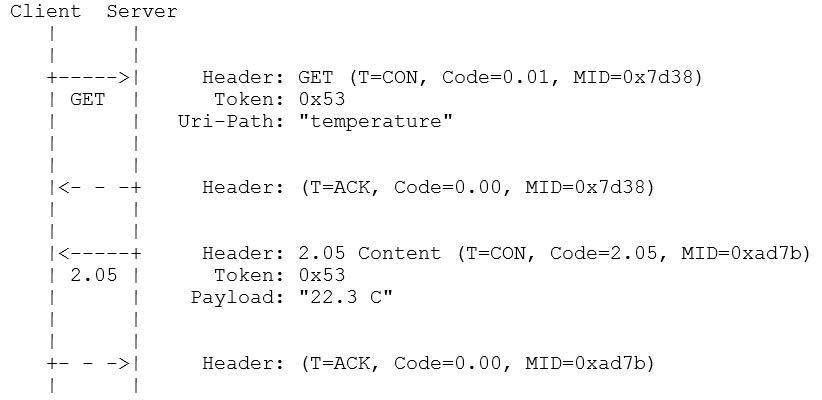
\includegraphics[width=\linewidth]{Images/Separate_response_confirmable_messages.jpg}
    \caption{Example of separate response with confirmable messages - Pay attention to the usage of the MID and Token fields.}
\end{figure}

\begin{figure}
    \centering
    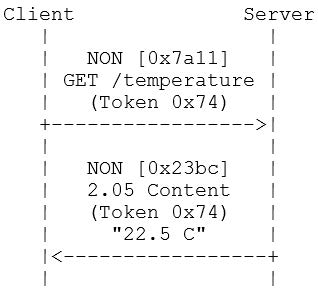
\includegraphics[width=0.5\linewidth]{Images/Separate_response_non_confirmable_messages.jpg}
    \caption{Example of separate response with non confirmable messages - In this case we have two different MIDs but the same token.}
\end{figure}

The separate response model is designed for situations where a server cannot respond immediately. For example, the request might trigger a long-running task or require fetching data from another source. In this case, making the client wait for a piggybacked response would be impractical.


This model involves a two-step process:

\begin{enumerate}
    \item Upon receiving the client's \textbf{CON} request, the server immediately sends back an empty \textbf{ACK} message. This message has the same Message ID as the request and serves only to confirm that the request was received, stopping the client from retransmitting.
    \item Later, when the server has finished processing and the response is ready, it sends this response to the client as a \textit{new} \textbf{CON} message. This new message contains the same \textbf{Token} as the original request, which allows the client to match this delayed response to its initial query. However, because it is a new CON message, it has a new, unique \textbf{Message ID}. Because the server's final response is a CON message, the client is obligated to send its own empty ACK to confirm its receipt, completing the transaction.
\end{enumerate}

\section{Client and Server Responsibilities in CoAP Message Correlation}

A frequent source of confusion when studying CoAP concerns the respective roles of the client and the server in request--response correlation, in particular with respect to the use of the Token field. This section clarifies these aspects and resolves common misconceptions related to piggybacked and separate responses.

\subsection{Stateless Nature of CoAP Interactions}

CoAP is a stateless protocol at the application layer: neither the client nor the server maintains implicit session state across multiple message exchanges. Each request is processed independently, and all information required to interpret a response must be contained within the messages themselves.

In particular, the server does \emph{not} remember previous requests when generating a response, nor does it rely on information stored across different interactions. Message correlation is therefore achieved exclusively through explicit protocol fields.

\subsection{Message ID and Token: Distinct Responsibilities}

CoAP provides two distinct mechanisms that serve different purposes:

\begin{itemize}
    \item \textbf{Message ID (MID)} is used for reliability and duplicate detection at the message layer. It allows a receiver to match a message with its corresponding acknowledgement (ACK) and to detect retransmissions.
    \item \textbf{Token} is used for request--response correlation at the application layer. It enables a client to associate a response with the request that triggered it, independently of the Message ID.
\end{itemize}

These two mechanisms are orthogonal: the Message ID supports reliable delivery, while the Token supports semantic correlation.

\subsection{Who Decides Whether to Use a Token}

The Token field is chosen by the \textbf{client} when generating a request. The client may select a Token Length (TKL) between 0 and 8 bytes. A value of \texttt{TKL = 0} indicates that no token is present.

Importantly, the client does \emph{not} need to know in advance whether the server will produce a piggybacked or a separate response. The decision to include or omit a token is based on whether the client expects ambiguity in correlating responses, not on the server’s internal processing time.

\subsection{When TKL = 0 Is Correct}

A request with \texttt{TKL = 0} is perfectly valid and common in simple interactions. This typically occurs when:

\begin{itemize}
    \item Only a single request is outstanding.
    \item A piggybacked response is expected.
    \item No proxies or observers are involved.
\end{itemize}

In this case, the response can be uniquely identified using the Message ID alone, and the Token would be redundant. This explains why instructional material and protocol examples often show messages with \texttt{TKL = 0}.

\subsection{When the Token Becomes Necessary}

The Token becomes necessary whenever Message IDs alone are insufficient to ensure unambiguous correlation. This includes, but is not limited to:

\begin{itemize}
    \item Separate responses, where the final response uses a different Message ID.
    \item Multiple concurrent requests issued by the same client.
    \item Interactions involving proxies.
    \item Long-lived relationships such as resource observation.
\end{itemize}

In these scenarios, the server simply echoes the Token received in the request back in the response, without interpreting its value. The semantic meaning of the Token exists entirely at the client side.

\subsection{Server Behavior and Processing Strategy}

The server does not infer or assume whether a request expects a piggybacked or a separate response. If the server is unable to generate a response immediately, it acknowledges the request and later sends a separate response using the same Token.

Crucially, the server does not require any prior knowledge of the client’s expectations, nor does the client need to retransmit the request purely because processing is delayed. CoAP’s design allows this flexibility without introducing implicit sessions or additional signaling.

\subsection{Design Implication}

The presence of messages with \texttt{TKL = 0} does not indicate an error or an incomplete interaction. Rather, it reflects CoAP’s minimalist philosophy: protocol fields are used only when they provide additional semantic value. Tokens are optional, but indispensable in scenarios where ambiguity would otherwise arise.

\section{Managing Unreliability: Handling Packet Loss}

CoAP's reliability mechanism is designed to gracefully handle the packet loss inherent in many wireless and constrained networks. \\

If a client's initial \textbf{CON} request is lost in transit, the client will never receive an ACK. Its timeout will expire, and it will retransmit the identical request, with the same Message ID and Token. (See figure ~\ref{fig:packet_loss_1}) \\

\begin{figure}
    \centering
    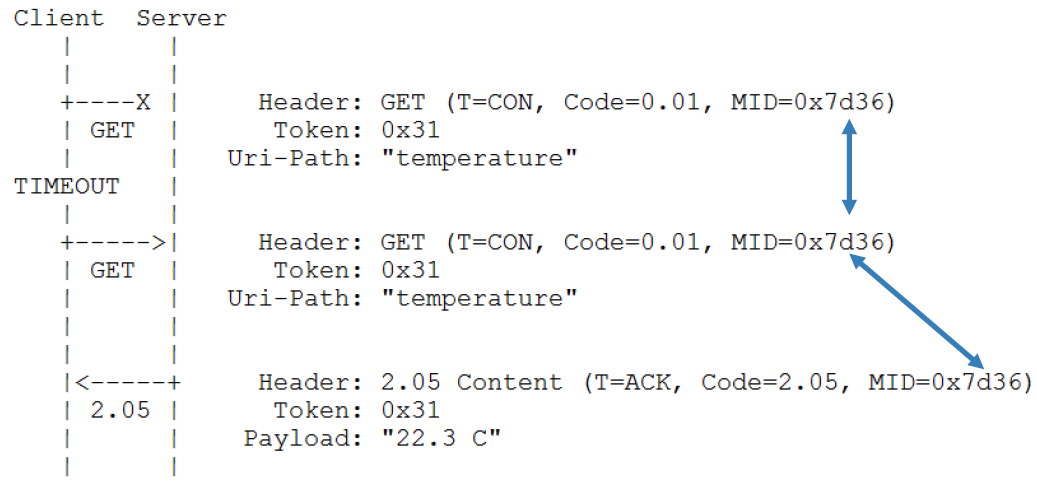
\includegraphics[width=\linewidth]{Images/Packet_loss_case_1.png}
    \caption{Client's CON request lost in transit}
    \label{fig:packet_loss_1}
\end{figure}

A more complex scenario occurs if the client's request is successfully delivered, but the server's \textbf{ACK} (which may contain a piggybacked response) is lost on the way back. From the client's perspective, this situation is indistinguishable from the first: it simply did not receive an acknowledgment. Consequently, the client will time out and retransmit the original request. When the server receives this duplicate request (which it identifies by the duplicate Message ID), it understands that its previous response was likely lost. It discards the duplicate request and simply retransmits its original response. (See figure ~\ref{fig:packet_loss_2})

\begin{figure}
    \centering
    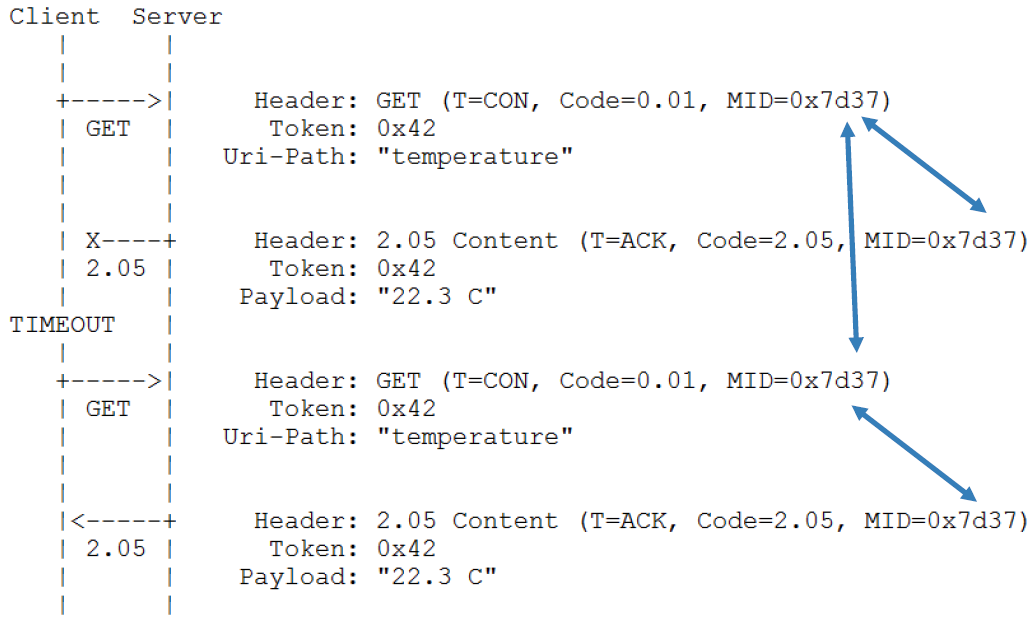
\includegraphics[width=\linewidth]{Images/Packet_loss_case_2.png}
    \caption{Server's ACK lost in transit}
    \label{fig:packet_loss_2}
\end{figure}

\chapter{Enhancing Efficiency: Caching and Proxying}

Similar to its counterpart HTTP, CoAP incorporates features designed to improve efficiency and reduce network load—objectives that are critically important in constrained environments. Caching resource representations and leveraging proxies are key strategies for minimizing bandwidth consumption and energy expenditure. This section analyzes CoAP's caching and proxying capabilities.

CoAP supports two primary caching mechanisms to reduce redundant data transmission:

\begin{enumerate}
    \item \textbf{Time-Based Freshness:} A server can include the \texttt{Max-Age} option in a response. This option defines the lifetime, in seconds, for which the resource representation should be considered "fresh" in a cache. A client or proxy can serve a cached response for subsequent requests within this lifetime without needing to contact the origin server.
    \item \textbf{Validity-Based Freshness:} A server can associate an \texttt{Etag} (Entity Tag) with a resource representation. When a client's cached copy with a specific \texttt{Etag} becomes stale, the client can send a new request to the server including that \texttt{Etag}. If the resource on the server has not changed, the server confirms its validity with a \texttt{2.03 Valid} response code and an empty body. This avoids the need to re-transmit the entire resource, thereby saving significant bandwidth.
\end{enumerate}

Proxies play an even more necessary role in CoAP networks than in traditional web environments. They are deployed for several key reasons:

\begin{itemize}
    \item To act as a centralized gateway on behalf of an entire network of constrained nodes.
    \item To support nodes that sleep for long periods to preserve energy, a strategy known as an "aggressive duty cycle".
    \item To reduce overall network load by aggregating requests or serving cached content.
\end{itemize}

CoAP architecture accommodates two primary types of proxies. The minority case is the "pure CoAP proxy," which operates solely within the CoAP protocol to enhance performance and manage network load as described above. A more prevalent and functionally distinct type is the "cross-proxy," or gateway, which is designed for interoperability.

A cross-proxy translates requests and responses between different protocols, most commonly between HTTP and CoAP. This enables seamless interoperability between the broader web and constrained CoAP networks. For example, an HTTP client can send a standard \texttt{GET} request to a cross-proxy. The proxy then translates this into a CoAP \texttt{GET} request, forwards it to the constrained CoAP server, receives the CoAP response, and translates it back into an HTTP response for the original client. This seamless translation makes CoAP resources accessible to standard web clients.

These efficiency features are crucial for general-purpose interactions, but CoAP also supports more advanced, application-specific patterns for M2M communication.

\begin{figure}
    \centering
    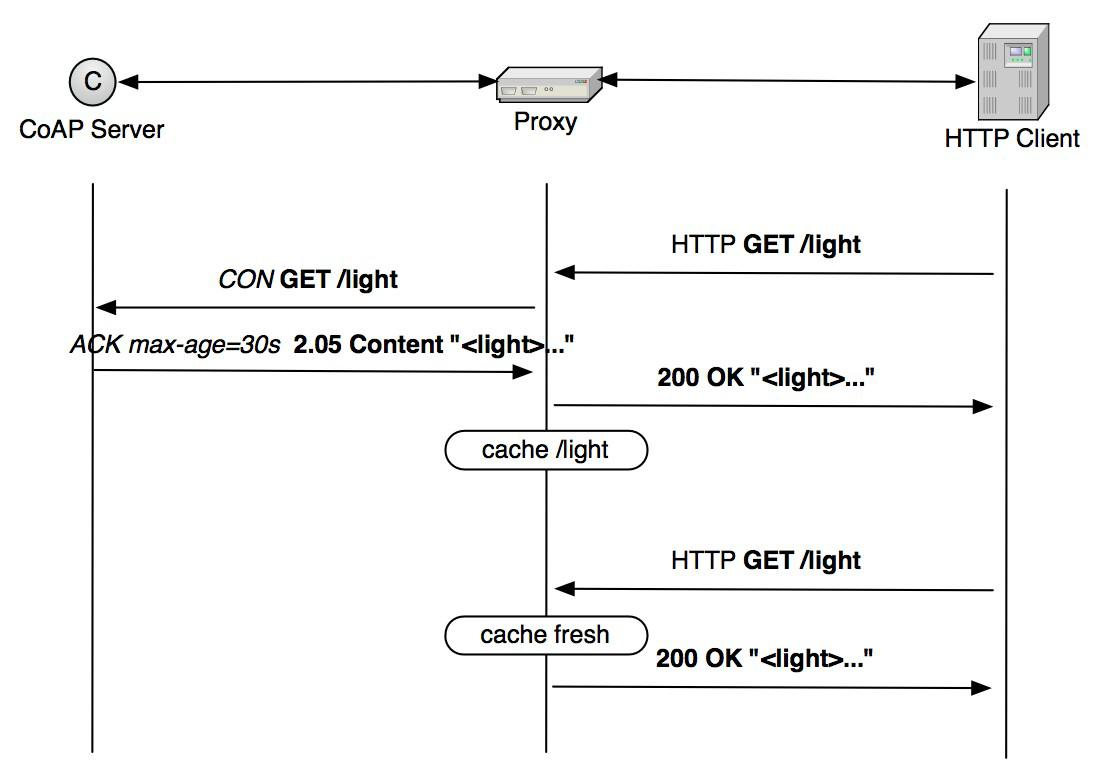
\includegraphics[width=\linewidth]{Images/Proxying_and_caching.jpg}
    \caption{CoAP proxying and caching}
    \label{fig:proxying_and_caching}
\end{figure}

\chapter{Advanced Interaction Patterns}

CoAP extends beyond a simple request-response model to support more sophisticated M2M interaction patterns that are essential for dynamic IoT applications like sensor networks and remote actuation. These patterns enable proactive data updates and efficient group management.

\section{Observe mechanism}

\begin{figure}
    \centering
    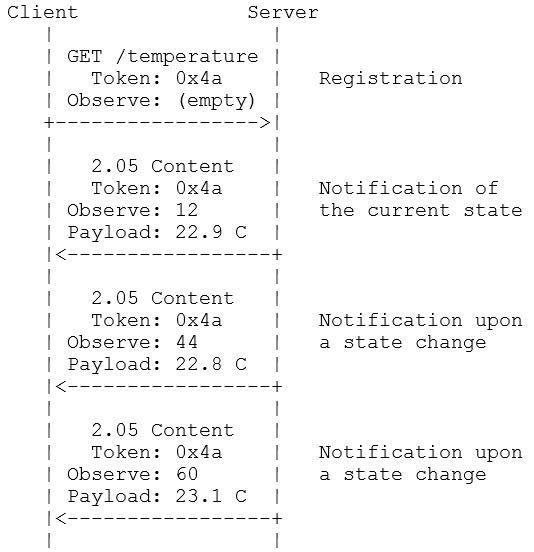
\includegraphics[width=\linewidth]{Images/Observing_a_resource.jpg}
    \caption{A client observing a resource in CoAP}
    \label{fig:client_observing_resource}
\end{figure}

A critical feature defined in RFC 7641 is the "observe" mechanism. This implements a publish/subscribe pattern that allows a client to be notified of changes to a resource's state without resorting to inefficient and resource-intensive polling. This is particularly valuable for monitoring sensor data that changes over time.

The observer workflow follows a clear, stateful process (See figure ~\ref{fig:client_observing_resource}):

\begin{enumerate}
    \item \textbf{Registration:} A client initiates the process by sending a \texttt{GET} request for a resource and includes the \texttt{Observe} option with a value of \texttt{0}. This signals to the server that the client wishes to register as an observer for that resource.
    \item \textbf{Initial Response:} The server processes the request and sends a response containing the current state of the resource. This response confirms the subscription by including the \texttt{Observe} option and establishes the \textit{baseline} for the Observe sequence number.
    \item \textbf{Notification:} Whenever the state of the observed resource changes, the server sends an unsolicited notification message to the client. This message contains the updated resource representation, the same Token from the original request because all the responses are related to it, and an incremented value in the \texttt{Observe} option. This sequence number, which begins incrementing with the first actual notification, ensures notifications are processed in the correct order.
    \item \textbf{Deregistration:} A client can cancel its observation in several ways: by rejecting a notification with a \texttt{Reset} message, by re-issuing a \texttt{GET} request for the same resource without the \texttt{Observe} option, or by issuing a \texttt{GET} with the \texttt{Observe} option set to \texttt{1} (deregister).
\end{enumerate}

While the observer pattern significantly reduces network traffic by eliminating polling, it introduces a small amount of overhead on the server, which must maintain a list of registered observers for each observable resource.

\begin{figure}
    \centering
    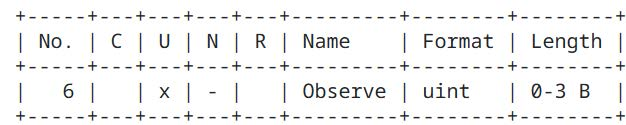
\includegraphics[width=\linewidth]{Images/Observe_option.jpg}
    \caption{CoAP observe option specification - This option is missing in figure ~\ref{fig:coap_option_flags}}
    \label{fig:observe_option_specification}
\end{figure}

\section{Group communication}

In addition to observing individual resources, CoAP also supports \textbf{Group Communication} by allowing a client to send a request to an IP multicast group. This powerful feature enables a single message to perform sensing or actuation commands on multiple nodes simultaneously. For instance, a client could send one \texttt{PUT} request to a multicast address to turn on or change the color of an entire group of smart lights. (See figure ~\ref{fig:group_communication}) \\

\begin{figure}
    \centering
    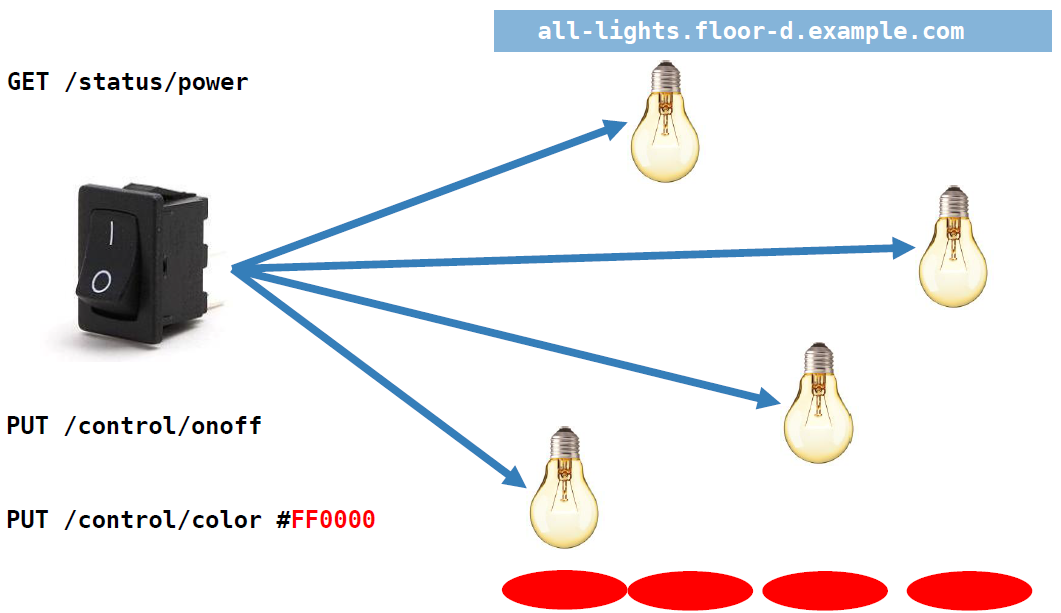
\includegraphics[width=\linewidth]{Images/Group_communication.png}
    \caption{CoAP group communication}
    \label{fig:group_communication}
\end{figure}

These advanced patterns provide the mechanisms to interact with known resources, but a fundamental challenge in M2M environments is discovering what resources are available in the first place.

\chapter{Resource Discovery with CoRE Link Format}

In the conventional web, users rely on powerful search engines to find resources. This model is unsuitable for M2M environments, where machines need an automated and lightweight way to discover services. To address this, the IETF designed a simple protocol specified in the CoRE Link Format (RFC 6690), enabling clients to discover the resources hosted on a constrained server. \\

This discovery protocol mirrors the classic distributed computing pattern seen in architectures like SOAP/UDDI, defining distinct roles for network participants: clients that use resources, providers that host them, and registries that maintain a catalog of available resources (See figure ~\ref{fig:client_registry_server_interaction}). A single node may act as both provider and registry, or these roles can be separate. \\

\begin{figure}
    \centering
    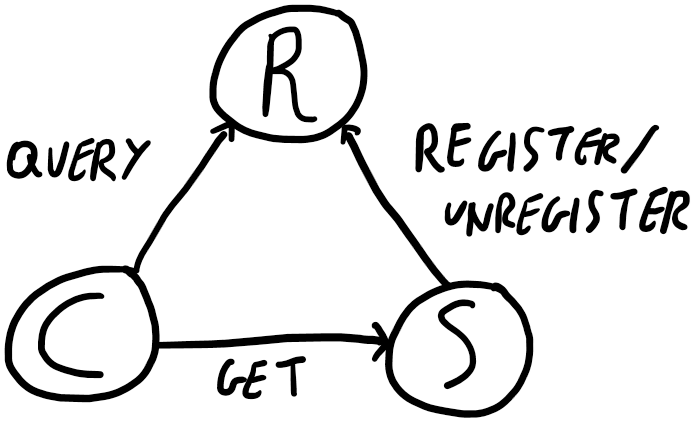
\includegraphics[width=0.5\linewidth]{Images/Client_Server_Registry.png}
    \caption{CoAP client-registry-server interaction}
    \label{fig:client_registry_server_interaction}
\end{figure}

This architecture enables two distinct use cases. First, a client can directly query a provider's resource catalog by sending a \texttt{GET} request to its well-known URI (\texttt{/.well-known/core}). Second, a resource provider can manage its listings on a separate resource directory (a registry) by using \texttt{POST} to register its resources and \texttt{DELETE} to unregister them. This separation of roles allows for the creation of centralized discovery services within a constrained network. \\

A key feature of the protocol is the ability for clients to filter the list of resources returned by a server. This is accomplished by including filter attributes in the Uri-Query option of a \texttt{GET} request, preventing the server from having to send a potentially large list of all its resources. This makes the CoRE Link Format not just a protocol but a tool for designing navigable and logical M2M resource hierarchies, as network designers can organize nodes and paths with the expectation that clients will use filtering and regular expressions for efficient discovery. \\

\begin{table}[h]
    \centering
    \begin{tabular}{|l|l|p{4cm}|l|}
        \hline
        \textbf{Attribute} & \textbf{Name} & \textbf{Description} & \textbf{Example Usage} \\
        \hline
        \texttt{href} & H-Ref / Path & Filters resources by their path on the server. Supports regular expressions. & \texttt{?href=sensor/*} \\
        \hline
        \texttt{rt} & Resource Type & Filters by an application-specific meaning or type, like "temperature-c". & \texttt{?rt=light*} \\
        \hline
        \texttt{if} & Interface Description & Filters by a name or URI that describes how to interact with the resource. & \texttt{if="sensor"} \\
        \hline
        \texttt{ct} & Content Type & Filters by the MIME content format of the resource. & \texttt{ct=40} (for a link-format list) \\
        \hline
        \texttt{sz} & Size & Filters by the estimated maximum resource size. & N/A in source \\
        \hline
    \end{tabular}
    \caption{CoRE Link Format Attributes}
\end{table}

To illustrate, a client might first send a \texttt{GET} request to \texttt{/.well-known/core}. The server could respond with \texttt{</sensors>;ct=40}, indicating a resource \texttt{/sensors}. The critical \texttt{ct=40} attribute signifies that this resource is itself a link-format list—effectively a folder. Understanding this, the client can then "drill down" by sending a second \texttt{GET} request to \texttt{/sensors}, which would return a list of specific sensor resources available at that path (e.g., \texttt{/sensors/temp} and \texttt{/sensors/light}). This hierarchical and filterable discovery process is essential for navigating services in complex M2M deployments. \\

With an understanding of the protocol's theory, the final step is to examine the practical tools available for its implementation.

\chapter{The CoAP Ecosystem: Tools and Implementations}

A robust ecosystem of open-source software libraries and developer tools supports the practical development, deployment, and debugging of CoAP-based applications. These resources are critical for accelerating the adoption of CoAP in the IoT landscape. \\

Numerous open-source implementations are available for a variety of programming languages and platforms, including:

\begin{itemize}
    \item \textbf{Java:} Popular libraries include \textbf{Californium} and \textbf{jCoAP}.
    \item \textbf{C:} Widely used C libraries are \textbf{Erbium} and \textbf{libCoAP}.
    \item \textbf{Embedded Operating Systems:} Native CoAP support is integrated into platforms like \textbf{TinyOS} and \textbf{Contiki}.
    \item \textbf{Platform-Specific Libraries:} Dedicated libraries are available for platforms like \textbf{Arduino}.
\end{itemize}

To aid in development and debugging, several tools provide a high-level interface for interacting with CoAP servers. Browser extensions, such as \textbf{Copper} for Firefox (See figure ~\ref{fig:copper}), offer a graphical user interface for crafting and sending CoAP requests and viewing responses, functioning much like the Postman tool does for HTTP APIs. When using such tools, the server URI is specified with the \texttt{coap://} scheme. \\

\begin{figure}
    \centering
    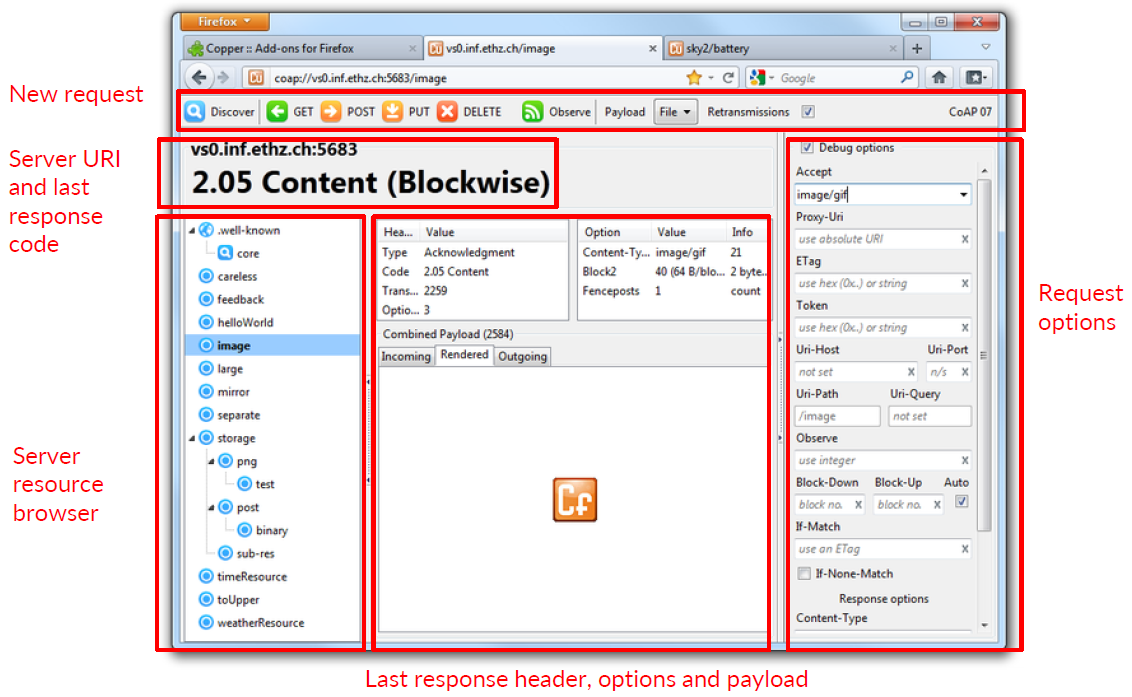
\includegraphics[width=\linewidth]{Images/Copper.png}
    \caption{Copper browser interface}
    \label{fig:copper}
\end{figure}

For deeper network-level debugging, network analysis tools like \textbf{Wireshark} include built-in support for the CoAP protocol. This allows developers to perform deep packet inspection on CoAP message exchanges, verifying message types, options, and payloads for troubleshooting complex interactions. This comprehensive suite of libraries and tools establishes CoAP as a practical and well-supported standard, solidifying its role as a foundational protocol for building scalable and efficient Internet of Things systems. \\

In conclusion, CoAP stands as a masterclass in protocol design for constrained environments. By meticulously engineering a compact binary format and delta-encoded options, it directly solves the \textbf{message verbosity} of HTTP. By building upon UDP with a tailored, application-layer reliability mechanism and offering dual interaction models, it provides robust M2M communication without the \textbf{implementation complexity} of a full TCP stack. Finally, through its built-in support for discovery and observation, it addresses the \textbf{feature mismatch} that makes HTTP cumbersome for the IoT. It is this synthesis of features that makes CoAP a robust and efficient protocol, perfectly suited for building a scalable and interoperable Web of Things.

\chapter{Client--Proxy--Server Interaction in CoAP}

CoAP is frequently deployed in heterogeneous network architectures where constrained devices are not directly reachable by traditional Internet clients. In such scenarios, a \emph{CoAP proxy} plays a fundamental role by translating requests and responses between different application-layer protocols, most commonly HTTP and CoAP.

This chapter illustrates a complete and coherent interaction involving an HTTP client, a CoAP proxy, and a CoAP server, using a temperature sensing service as a running example.

\section{Scenario Description}

Assume a constrained device exposes a temperature sensor through the resource:

\[
/sensors/temperature
\]

The device supports query parameters that allow the client to specify the unit of measurement and the desired precision.

An external client issues the following HTTP request:

\begin{verbatim}
GET http://example.com:400/sensors/temperature?unit=celsius&precision=high
\end{verbatim}

The client is unaware of CoAP and communicates only with an HTTP endpoint. The domain \texttt{example.com} and port \texttt{400} identify an HTTP-to-CoAP proxy.

\section{Role of the CoAP Proxy}

The proxy acts as an application-layer intermediary. Its responsibilities include:

\begin{itemize}
    \item receiving HTTP requests from clients;
    \item parsing the HTTP method, URI, and query parameters;
    \item translating the HTTP request into an equivalent CoAP request;
    \item forwarding the CoAP request to the appropriate CoAP server;
    \item translating the CoAP response back into an HTTP response.
\end{itemize}

The proxy does not maintain application-level session state between client and server. Each request is handled independently.

\section{Translation of the HTTP Request}

Upon receiving the HTTP request, the proxy parses the URI and decomposes it into its logical components:

\begin{itemize}
    \item Scheme: \texttt{http}
    \item Host: \texttt{example.com}
    \item Port: \texttt{400}
    \item Path segments: \texttt{sensors}, \texttt{temperature}
    \item Query parameters: \texttt{unit=celsius}, \texttt{precision=high}
\end{itemize}

The proxy then constructs a CoAP \texttt{GET} request. Instead of embedding the URI as a textual string, it encodes each component using CoAP options.

\section{Construction of the CoAP Request}

The resulting CoAP request contains the following elements:

\begin{itemize}
    \item \textbf{Header}: specifying version, message type, and code (\texttt{GET});
    \item \textbf{Token}: used to correlate request and response;
    \item \textbf{Options}: representing the URI components;
    \item \textbf{Payload}: empty for a \texttt{GET} request.
\end{itemize}

The sequence of URI-related options is:

\begin{itemize}
    \item \texttt{Uri-Host = example.com}
    \item \texttt{Uri-Port = 400}
    \item \texttt{Uri-Path = sensors}
    \item \texttt{Uri-Path = temperature}
    \item \texttt{Uri-Query = unit=celsius}
    \item \texttt{Uri-Query = precision=high}
\end{itemize}

These options are encoded in strictly increasing order of their option numbers and transmitted using delta encoding.

\section{Reception and Parsing at the CoAP Server}

The CoAP server receives the binary message over UDP. From the server’s perspective, there is no notion of HTTP, URLs, or proxies. The server processes only the CoAP message structure.

During option parsing, the server:

\begin{enumerate}
    \item initializes the current option number to zero;
    \item reads each option sequentially;
    \item reconstructs the full option number by adding the received delta;
    \item interprets the option value according to the option type.
\end{enumerate}

This process is entirely local to the received message and does not require any stored state from previous interactions.

\section{Resource Identification and Request Interpretation}

After parsing the options, the server reconstructs the logical request target. The \texttt{Uri-Path} options identify the resource:

\[
/sensors/temperature
\]

The \texttt{Uri-Query} options are interpreted as request parameters that influence how the resource is accessed or represented. In this example, they specify that the temperature should be returned in Celsius with high precision.

Importantly, the server does not infer missing information and does not rely on implicit context. The complete meaning of the request is derived exclusively from the options present in the message.

\section{Response Generation}

The server accesses the temperature sensor, retrieves the current measurement, and generates a CoAP response message. The response typically includes:

\begin{itemize}
    \item a response code (e.g., \texttt{2.05 Content});
    \item the same token used in the request;
    \item optional response options (e.g., \texttt{Content-Format});
    \item a payload containing the temperature value.
\end{itemize}

The response is sent back to the proxy using UDP.

\section{Translation of the Response}

Upon receiving the CoAP response, the proxy matches it to the original HTTP request using the token. It then translates the CoAP response into an HTTP response, mapping:

\begin{itemize}
    \item the CoAP response code to an HTTP status code;
    \item the payload to the HTTP response body;
    \item relevant CoAP options to HTTP headers.
\end{itemize}

The HTTP response is finally delivered to the client, which remains unaware that the request was served by a constrained CoAP device.

\section{Conclusion}

This interaction highlights several fundamental design principles of CoAP:

\begin{itemize}
    \item the protocol is strictly stateless at the application level;
    \item all request semantics are explicitly encoded in each message;
    \item URI decomposition into options enables compact encoding and efficient parsing;
    \item proxies can transparently bridge CoAP with other application-layer protocols.
\end{itemize}

As a result, CoAP achieves interoperability with the Web while remaining lightweight enough for constrained IoT environments.

\end{document}
